\documentclass{article}
\usepackage{geometry}
\geometry{paperwidth=21cm,
paperheight=29.7cm,
margin=1cm}
\usepackage{amsmath}
\usepackage{mathfmv}
\usepackage{siunitx}
\usepackage{pgf}
\usepackage{tikz}
\usepackage{pgfplots}
\pgfplotsset{compat=1.18}
\begin{document}
\[
\boldsymbol{H(p)=\dfrac{p^2}{0.3\cdot10^{-9}p^2+1}}
\]
\begin{center}
\begin{tikzpicture}[trim axis left]
\begin{axis}[ticklabel style = {font=\normalsize},
width=0.9\textwidth,
height=0.25\textheight,
grid=both,
major grid style={black!40},
label style={font=\large},
xmode=log,ymode=normal,
xlabel={},
ylabel={Gain (\si{\decibel})},
xtick={1,10,100,1000,10000,100000,1000000,10000000,100000000,1000000000},
ytick={60,78,96,114,132,150,168,186,204,222,240},
xticklabels={$10^{0}$,$10^{1}$,$10^{2}$,$10^{3}$,$10^{4}$,$10^{5}$,$10^{6}$,$10^{7}$,$10^{8}$,$10^{9}$},
yticklabels={60,78,96,114,132,150,168,186,204,222,240},
xmin=1,xmax=1000000000,
ymin=60,ymax=240]
\addplot[ultra thick, blue,domain=1:1000000000,samples=256]{189.54242509439325+40*log10(x)-10*log10(0.0+(x+(54772.255750516604))*(x+(54772.255750516604)))-10*log10(0.0+(x+(-54772.255750516604))*(x+(-54772.255750516604)))};
\addplot[line width=2pt,red,dashed,domain=1:54772.255750516604, samples=16]{0.0+40*log10(x)};
\addplot[line width=2pt,red,dashed,domain=54772.255750516604:1000000000, samples=16]{0.0+40*log10(x)+(-40.0)*log10(x/54772.255750516604)};
\end{axis}
\end{tikzpicture}

\begin{tikzpicture}[trim axis left]
\begin{axis}[ticklabel style = {font=\normalsize},
width=0.9\textwidth,
height=0.25\textheight,
grid=both,
major grid style={black!40},
label style={font=\large},
xmode=log,ymode=normal,
xlabel={Pulsation (\si{\radian\per\second})},
ylabel={Phase (\si{degree})},
xtick={1,10,100,1000,10000,100000,1000000,10000000,100000000,1000000000},
ytick={-90,-72,-54,-36,-18,0,18,36,54,72,90},
xticklabels={$10^{0}$,$10^{1}$,$10^{2}$,$10^{3}$,$10^{4}$,$10^{5}$,$10^{6}$,$10^{7}$,$10^{8}$,$10^{9}$},
yticklabels={-90,-72,-54,-36,-18,0,18,36,54,72,90},
xmin=1,xmax=1000000000,
ymin=-90,ymax=90]
\addplot[ultra thick, blue,domain=1:1000000000,samples=256]{180+(-2)*atan2(x/54772.255750516604,1)};
\addplot[line width=2pt,red,dashed,domain=1:54772.255750516604,samples=16]{180};
\draw[line width=2pt,red,dashed](axis cs:54772.255750516604,180) -- (axis cs:54772.255750516604,0.0);
\addplot[line width=2pt,red,dashed,domain=54772.255750516604:1000000000,samples=16]{0.0};
\end{axis}
\end{tikzpicture}
\end{center}
\paragraph{Fonctions réelles du gain et du déphasage}
\[
G(\omega)=|H(\jw)|=\dfrac{2999999999\left(- \omega^{2}\right)}{1 - \frac{333333333333333 \omega^{2}}{1000000000000000000000000}}
\]
\[
G_{dB}(\omega)=189+40\log\omega-20\log{\left(1+\left(\frac{\omega}{\omega_1}\right)^2\right)}
\]
\[
\phi(\omega)=\arg{H(\jw)}=180-2\arctan{\left(\frac{\omega}{\omega_1}\right)}
\]
\paragraph{Quelques valeurs particulières calculées}
\begin{center}
\begin{tabular}{ccc}
\hline
$\omega$ (\si{\radian\per\second}) & Gain (\si{\decibel}) & Phase (\si{\degree})\\
\hline
     1.00000 &      0.00000 &   -180.00000\\
\hline
     7.94328 &     36.00000 &   -180.00000\\
\hline
    63.09573 &     72.00001 &   -180.00000\\
\hline
   501.18723 &    108.00073 &   -180.00000\\
\hline
  3981.07171 &    144.04601 &   -180.00000\\
\hline
 31622.77660 &    183.52183 &   -180.00000\\
\hline
\textbf{ 54772.25575} & \textbf{   404.60715} & \textbf{  -360.00000}\\
\hline
251188.64315 &    189.96555 &   -360.00000\\
\hline
1995262.31497 &    189.54897 &   -360.00000\\
\hline
15848931.92461 &    189.54253 &   -360.00000\\
\hline
125892541.17942 &    189.54243 &   -360.00000\\
\hline
1000000000.00000 &    189.54243 &   -360.00000\\
\hline
\end{tabular}
\end{center}
\end{document}
